\section{Vision}

Although the main intent of the vision was to detect the given set of objects (see figure \ref{fig:object_set},
it was later on also used to exploit wall and ground information for mapping and localization functionality.

\begin{figure}
\begin{center}
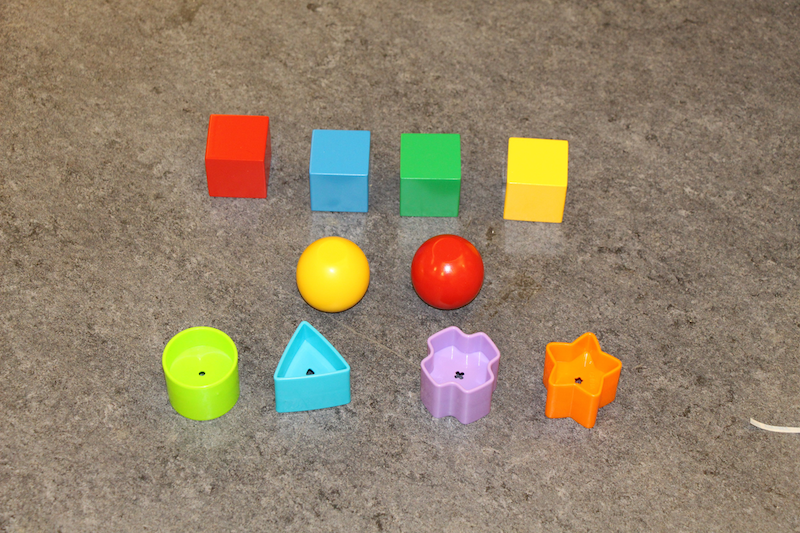
\includegraphics[width=0.38\textwidth]{figures/object_dataset}
\end{center}
\caption{Object data set}
\label{fig:object_set}
\end{figure}

\subsection{Object detection}

It was decided upon using the 3D information from the primesense to reduce susceptibility to illumination changes and to gain more information about the structure of objects.
Processing of the point cloud is mostly done with using the library \textit{Point Cloud Library}.
The detection and recognition can be divided in 4 different steps (see figure \ref{fig:vision:obj_det}).

\begin{itemize}
\item \textbf{Calibration:}
Takes the ground plane from the segmented planes and calculates the camera pitch and height.
\item \textbf{Transformation and subsampling:}
Receives a calibration matrix from the calibration and transforms the point cloud accordingly.
Simultaneously it downsamples the point cloud to reduce the number of points and so increase the processing speed in later steps.
\item \textbf{Plane segmentation:}
Takes in the subsampled point cloud and downsamples it even further so that only 1500 points are left.
Instead of using the regular approach of using voxel grid downsampling, offered by the PCL library,
the downsampling is performed by randomly picking 1500 points.
This is sufficient to have enough features on the planes.
RANSAC is applied to find all planes, until only a fraction of points is left unclassified (see result in figure \ref{fig:vision:seg_planes}).
To make use of the planes in mapping this step also calculates the oriented bounding box that the points on the plane encompasses.
Because two walls can lie on the same plane, a cluster segmentation is necessary to make the distinction.
The embedded euclidean cluster extraction turned out to be very expensive.
It was therefore decided to implement a 1D cluster segmentation. 
This can be achieved by projecting all points on the orthogonal vector of the planes normal vector, sorting them and finding gaps.
\item \textbf{ROI extraction:}
Takes in the segmented planes and removes all points in the point cloud that lie on that plane with regard to some distance threshold.
Euclidean cluster extraction, as implemented in the PCL library is applied to find clusters. 
Clusters that contain points lieing outside a given distance to the ground plane are immidiately dismissed.
The remaining clusters define the regions of interests (ROIs) and can be used for further processing.
\end{itemize}

\begin{figure}
\centering
\begin{subfigure}[b]{1.0\textwidth}
\centering
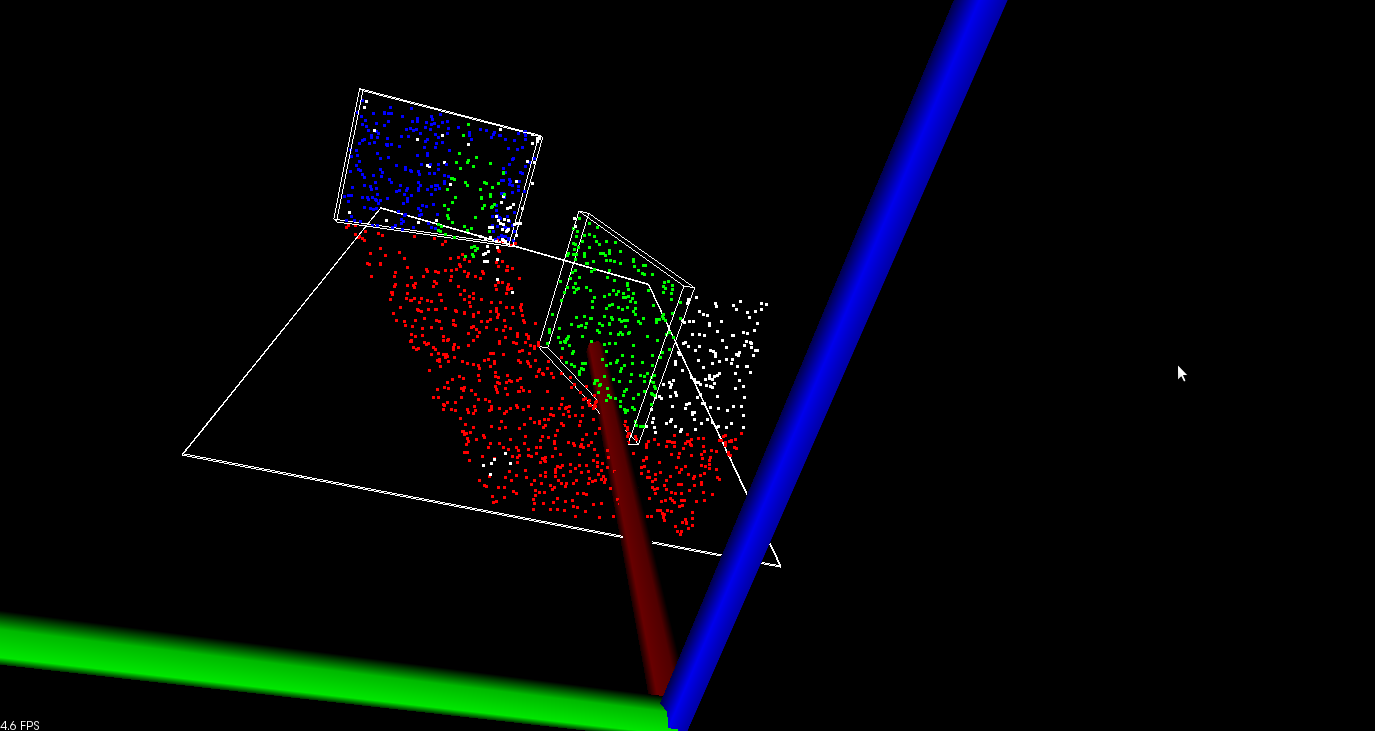
\includegraphics[width=0.8\textwidth]{figures/vision_planes.png}
\caption{Segmented planes. \textbf{Green:} Case when two unconnected walls are interpreted as one plane. Only the largest part is taken. \textbf{White:} Non segmented points.}
\label{fig:vision:seg_planes}
\vspace{10pt}
\end{subfigure}
\begin{subfigure}[b]{1.0\textwidth}
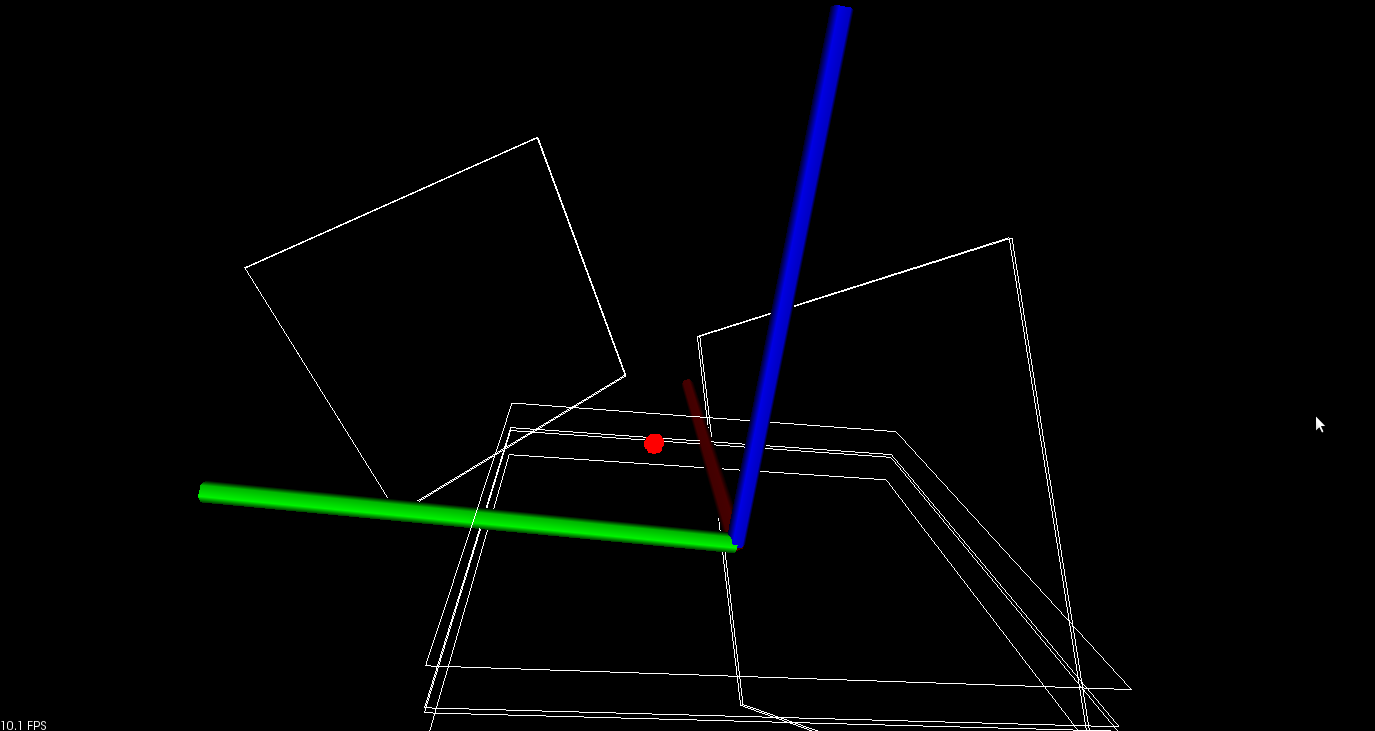
\includegraphics[width=0.8\textwidth]{figures/vision_roi_ball.png}
\centering
\caption{Segmented regions of interest. \textbf{Red:} ROI of a sphere. \textbf{Skewed rectangles:} Planes from (a). \textbf{Bottom sandwich:} Ground plane and maximum distance for accepting a cluster as a region of interest.}
\label{fig:vision:seg_rois}
\end{subfigure}
\caption{Results of the object detection}

\end{figure}

\begin{figure}
\begin{center}
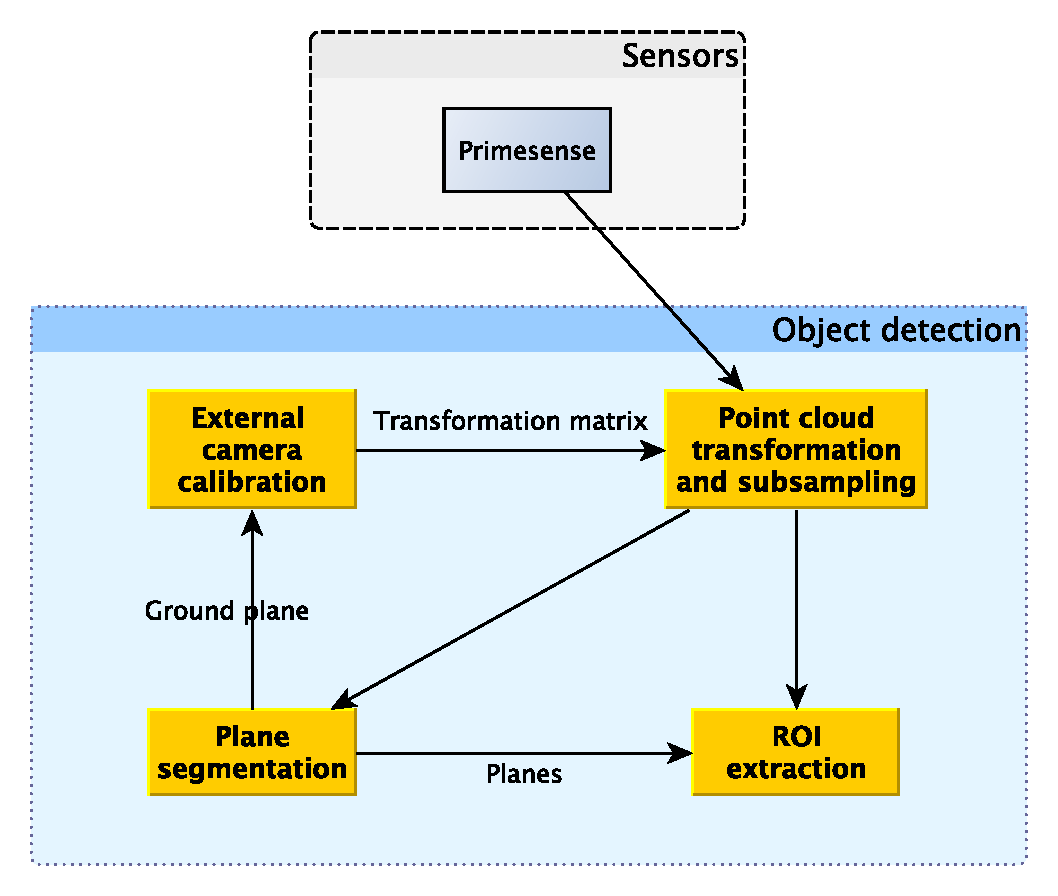
\includegraphics[width=0.45\textwidth]{figures/arch_vision_obj_det.pdf}
\end{center}
\caption{Object detection - Process flow}
\label{fig:vision:obj_det}
\end{figure}
 
\subsection{Object recognition} 
 
\subsection{Shape Recognition}

In this section we explain our logic behind the shape recognition algorithm.
The general idea was again model fitting.
We know about 3 very specific models that we want to try, cube, cylinder and sphere, and we have two objects with no general model.
The PCL library has available the RANSAC algorithm to fit some predifined models, like planes, spheres and cylinders. 
And that is what we used. 
The sphere fitting and cylinder are straightforward since they work exactely like the plane fitting mentioned above, the only difference being that the model is no longer a plane.
Hence they work in similar way as the plane fitting.
The big difference is the cube.
To recognize a cube we do plane fitting too, but we impose some conditions of the planes.

\begin{enumerate}
\item if 3 planes are detected then it's a cube
\item there has to be a parallel plane relative to the ground
\item distance between the ground plane and the parallel plane described above must be reasonable
\item the furthest plane must be the parallel plane
\end{enumerate}

The constraints above limit the possibility of noise being misclassified, as well as other shapes being mischaracterized.
There was obviously some empirical testing in order to find the best parameters for the RANSAC model fitting, like: 

\begin{itemize}
\item MAX:: I know some of them but can't remember their function
\end{itemize}


\subsection{Color Recognition}

Extracting the color values from an image, or in our case from points, is not a hard task. 
However, to give meaning to those values is harder, since the color itself depends on a rather large number of factors like available light, its intensity, its color, among others.
This makes it hard to obtain a robust but consistent color recognition algorithm.
Our approach was very empirical. The analysis is made per color possible and not all at once, even though the algorithm is the same whatever the color.
We started by analising the HSV (hue, saturation, value) values we got from the regions of interest, mainly the hue, which is what defines the color. 
We then tried to find meaning in those values, mainly their average.
We concluded that for the most part, the overall average of hues of all the points in the region of interest would be enough to obtain a good estimate of the color. 
So we defined an area our each color mean value around which the color will be.
The bigger the margin, the more robust the algorithm would be.
However, because of the specific colors, the margin could not be too large, or the added robustness would not be reliable, as colors would start to mix.
Because different conditions may lead to very different results, we weighted two times the previous result based on specific situations, mainly, the percentage of points that have the color being tested relative to the total number of points, and the probability of being of the color being analysed, i.e., considering the point clouds don't usually have that many points, we give a higher weight to probabilities above a certain value.
Because the blob of interest may have points not only belonging to the object we want, but also from the ground or wall (if the object is very close to one), the number of points that have a color similar to orange, color of the ground, is also relevant in deciding the true color of the object, and hence helps in determining the weight of the probability of the color being analysed.
The end result is a somewhat robust algorithm and consistent as far as our testing went. 

\begin{figure}
\begin{center}
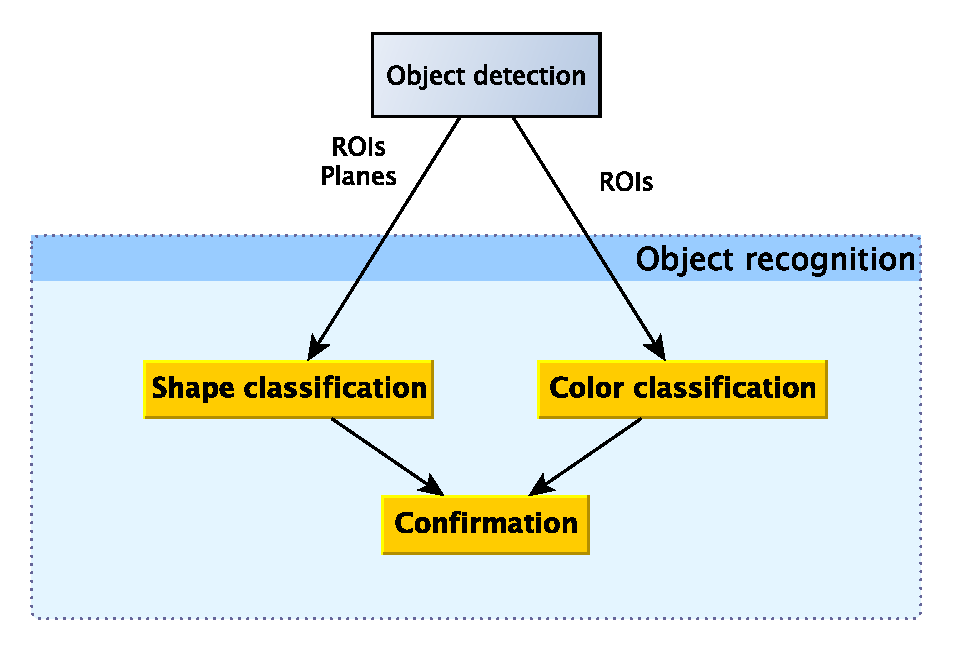
\includegraphics[width=0.45\textwidth]{figures/arch_vision_obj_rec.pdf}
\end{center}
\caption{Object recognition - Process flow}
\label{fig:vision:obj_rec}
\end{figure}